% ! Author = Omar Iskandarani
% ! Title  = Chirality as Time Asymmetry: A Swirl--String Theory Interpretation of Attosecond Photoionization Delays
% ! Date   = Sept 8, 2025
% ! Affiliation = Independent Researcher, Groningen, The Netherlands
% ! License = © 2025 Omar Iskandarani. All rights reserved.

\documentclass[reprint, aps, prl, longbibliography]{revtex4-2}
\usepackage[utf8]{inputenc}
\usepackage[T1]{fontenc}
\usepackage{graphicx}
\usepackage{amsmath,amssymb,amsfonts,bm}
\usepackage{siunitx}
\usepackage{subcaption}
\usepackage{booktabs}
\usepackage{hyperref}
\hypersetup{colorlinks=true,linkcolor=blue,citecolor=blue,urlcolor=blue}

\usepackage{tikz}
\usepackage{pgfplots}
\pgfplotsset{compat=1.18}
\usetikzlibrary{arrows.meta,calc,decorations.markings,positioning}
\usetikzlibrary{fpu}

% ==== Swirl String Theory (SST) macros ====
\newcommand{\swirlarrow}{%
    \mathchoice{\mkern-2mu\scriptstyle\boldsymbol{\circlearrowleft}}%
    {\mkern-2mu\scriptstyle\boldsymbol{\circlearrowleft}}%
    {\mkern-2mu\scriptscriptstyle\boldsymbol{\circlearrowleft}}%
    {\mkern-2mu\scriptscriptstyle\boldsymbol{\circlearrowleft}}%
}
\newcommand{\swirlarrowcw}{%
    \mathchoice{\mkern-2mu\scriptstyle\boldsymbol{\circlearrowright}}%
    {\mkern-2mu\scriptstyle\boldsymbol{\circlearrowright}}%
    {\mkern-2mu\scriptscriptstyle\boldsymbol{\circlearrowright}}%
    {\mkern-2mu\scriptscriptstyle\boldsymbol{\circlearrowright}}%
}

% Canonical symbols
\newcommand{\vswirl}{\mathbf{v}_{\swirlarrow}}
\newcommand{\vswirlcw}{\mathbf{v}_{\swirlarrowcw}}
\newcommand{\SwirlClock}{S_{(t)}^{\ \swirlarrow}}
\newcommand{\SwirlClockcw}{S_{(t)}^{\ \swirlarrowcw}}
\newcommand{\vnorm}{\lVert \vswirl \rVert}
\DeclareSIUnit\angstrom{\text{\AA}}

% ---- Local bibliography (self-contained build) ----
\begin{filecontents*}{refs.bib}
@article{Han2025,
  author  = {Han, M. and Ji, J.-B. and Blech, A. and Goetz, R. E. and Allison, C. and Greenman, L. and Koch, C. P. and W\"orner, H. J.},
  title   = {Attosecond control and measurement of chiral photoionization dynamics},
  journal = {Nature},
  year    = {2025},
  doi     = {10.1038/s41586-025-09455-4},
  note    = {online 27 Aug 2025}
}
@article{IskandaraniSSTCanon,
  author  = {Iskandarani, Omar},
  title   = {Swirl String Theory (SST) Canon v0.4.0},
  journal = {Zenodo},
  year    = {2025},
  doi     = {10.5281/zenodo.17052966},
  note    = {Foundational document for the SST framework}
}
@article{Krausz2009,
  author  = {Krausz, Ferenc and Ivanov, Misha},
  title   = {Attosecond physics},
  journal = {Rev. Mod. Phys.},
  volume  = {81},
  pages   = {163--234},
  year    = {2009},
  doi     = {10.1103/RevModPhys.81.163}
}
@article{Beaulieu2018,
  author  = {Beaulieu, S. and others},
  title   = {Attosecond-resolved photoionization of chiral molecules},
  journal = {Science},
  volume  = {358},
  pages   = {1288--1294},
  year    = {2018},
  doi     = {10.1126/science.aao5624}
}
@article{Demekhin2018,
    author = {Demekhin, Philipp V. and others},
    title = {Photoelectron circular dichroism in attosecond pump-probe experiments on chiral molecules},
    journal = {Phys. Rev. A},
    volume = {98},
    pages = {023421},
    year = {2018},
    doi = {10.1103/PhysRevA.98.023421}
}
@article{Pazourek2015,
  author  = {Pazourek, R. and Nagele, S. and Burgd\"orfer, J.},
  title   = {Attosecond chronoscopy of photoemission},
  journal = {Rev. Mod. Phys.},
  volume  = {87},
  pages   = {765--802},
  year    = {2015},
  doi     = {10.1103/RevModPhys.87.765}
}

@article{Dahlstrom2012,
  author  = {Dahlstr\"om, J. M. and L'Huillier, A. and Maquet, A.},
  title   = {Introduction to attosecond delays in photoionization},
  journal = {J. Phys. B},
  volume  = {45},
  pages   = {183001},
  year    = {2012},
  doi     = {10.1088/0953-4075/45/18/183001}
}
\end{filecontents*}


\begin{document}

\title{Chirality as Time Asymmetry: A Swirl--String Theory Interpretation of Attosecond Photoionization Delays}
\author{Omar Iskandarani}
\affiliation{Independent Researcher, Groningen, The Netherlands}
\date{September 8, 2025}

\begin{abstract}
Han \emph{et al.} (Nature, 2025) report enantiomer-dependent photoemission delays in gas-phase methyloxirane, with angle-resolved values reaching \SI{240}{\atto\second}. Here we sketch an interpretation in the Swirl--String Theory (SST) picture, where chirality carries a local, direction-sensitive time rate (“Swirl Clock”). Simple estimates map the reported delays to Å-scale effective path differences for the outgoing electron. While this is not a unique explanation—Coulomb–laser coupling and continuum–continuum phases remain plausible contributors—the SST view organizes the observations into a single, testable statement: reversing the Swirl Clock orientation should flip the forward/backward delay. We outline measurements that could falsify the proposal and note where present assumptions are likely to break.
\end{abstract}


\maketitle


\section{Introduction}
Attosecond spectroscopy now resolves the time scales on which chirality leaves a dynamical imprint \cite{Krausz2009,Beaulieu2018}. In methyloxirane, Han \emph{et al.} \cite{Han2025} find robust forward–backward (FB) photoemission delays whose sign tracks molecular handedness.

Our aim is modest: to ask whether these features admit a compact reading within Swirl--String Theory (SST) \cite{IskandaraniSSTCanon}. In SST, localized circulation fields endow matter with a direction-dependent “clock,” and chirality becomes a statement about that clock’s orientation. The idea is admittedly unconventional; nonetheless, it makes a sharp prediction about FB delays that can be checked without adopting the rest of the framework. We also point out where the SST reading likely fails and how such failures would look in data.


\section{Summary of Han et al. (2025)}
Using circularly polarized attosecond pulse trains in a RABBIT geometry, Han \emph{et al.} \cite{Han2025} report:
(i) an FB time delay of about \SI{60}{\atto\second} with sign reversal between enantiomers;
(ii) an angle-dependent spread up to \SI{240}{\atto\second}; and
(iii) a \SI{60}{\atto\second} offset in continuum–continuum paths.
These observations suggest a directional temporal structure that survives the ionization step.

\section{Swirl--String Theory and the Swirl Clock}
SST models elementary excitations as quantized circulation in a universal swirl medium \cite{IskandaraniSSTCanon}. We use only a minimal subset here. The “Swirl Clock,” $\SwirlClock$, encodes a local, direction-sensitive time rate modulated by the swirl speed $\vnorm$,
\begin{equation}
  dt_{\text{local}} = dt_{\infty}\,\sqrt{1 - \frac{\vnorm^2}{c^2}}.
\end{equation}
Opposite enantiomers are represented by opposite clock orientations ($\SwirlClock$ vs.\ $\SwirlClockcw$). In this stripped-down version we avoid detailed potential reconstructions and focus on the sign structure and scaling expectations relevant for FB delays.


% Combined figure with subcaptions
\begin{figure}[t]
    \centering
    \begin{subfigure}[b]{0.48\textwidth}
        \centering
        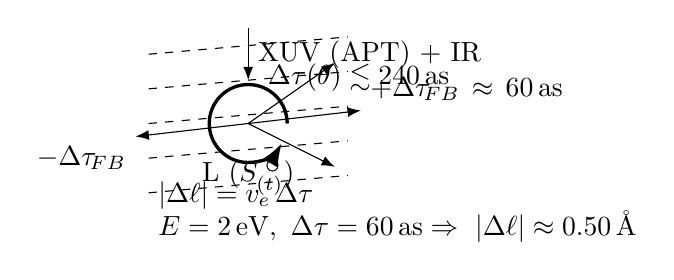
\begin{tikzpicture}[x=1cm,y=1cm,>=Latex, scale=0.55]
            \begin{scope}[shift={(0,0)}]
              \foreach \y in {-1.6,-0.8,0,0.8,1.6} \draw[dashed] (-2.3,\y) -- (2.3,\y+0.4);
              \draw[very thick,->] (0.9,0) arc[start angle=0,end angle=330,radius=0.9];
              \node at (0,-1.25) {L ($\SwirlClock$)};
              \draw[->] (0,2.2) -- (0,1.0) node[midway,right] {XUV (APT) + IR};
              \draw[->] (0,0) -- (2.6,0.3) node[above right] {$+\Delta\tau_{\!FB}\,\approx\,\SI{60}{as}$};
              \draw[->] (0,0) -- (-2.6,-0.3) node[below left] {$-\Delta\tau_{\!FB}$};
              \draw[->] (0,0) -- (2.0,1.4);
              \draw[->] (0,0) -- (2.0,-1.0);
              \node[align=left] at (2.55,1.05) {$\Delta\tau(\theta)\lesssim\SI{240}{as}$};
              \node[align=left,anchor=west] at (-2.3,-2.05) {$|\Delta\ell|=v_e\,\Delta\tau$\\$E=\SI{2}{eV},\ \Delta\tau=\SI{60}{as}\Rightarrow\ |\Delta\ell|\approx\SI{0.50}{\angstrom}$};
            \end{scope}
        \end{tikzpicture}
        \caption{L enantiomer with $+\Delta\tau_{\!FB}$.}
        \label{fig:enantiomer-l}
    \end{subfigure}
    \hfill
    \begin{subfigure}[b]{0.48\textwidth}
        \centering
        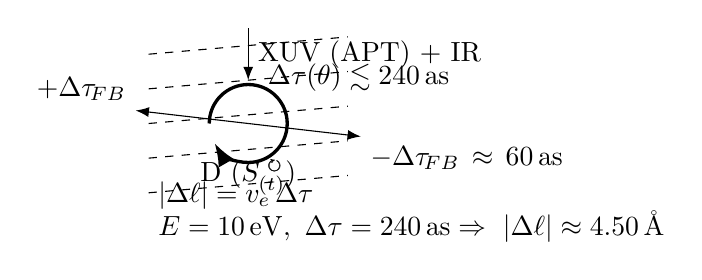
\begin{tikzpicture}[x=1cm,y=1cm,>=Latex, scale=0.55]
            \begin{scope}[shift={(0,0)}]
              \foreach \y in {-1.6,-0.8,0,0.8,1.6}
              \draw[dashed] (-2.3,\y) -- (2.3,\y+0.4);
              \draw[very thick,->] (-0.9,0) arc[start angle=180,end angle=-150,radius=0.9];
              \node at (0,-1.25) {D ($\SwirlClockcw$)};
              \draw[->] (0,2.2) -- (0,1.0) node[midway,right] {XUV (APT) + IR};
              \draw[->] (0,0) -- (2.6,-0.3) node[below right] {$-\Delta\tau_{\!FB}\,\approx\,\SI{60}{as}$};
              \draw[->] (0,0) -- (-2.6,0.3) node[above left] {$+\Delta\tau_{\!FB}$};
              \node[align=left] at (2.55,1.05) {$\Delta\tau(\theta)\lesssim\SI{240}{as}$};
              \node[align=left,anchor=west] at (-2.3,-2.05) {$|\Delta\ell|=v_e\,\Delta\tau$\\$E=\SI{10}{eV},\ \Delta\tau=\SI{240}{as}\Rightarrow\ |\Delta\ell|\approx\SI{4.50}{\angstrom}$};
            \end{scope}
        \end{tikzpicture}
        \caption{D enantiomer with $-\Delta\tau_{\!FB}$.}
        \label{fig:enantiomer-d}
    \end{subfigure}
    \caption{Schematic of Swirl Clock–induced delays for (a) L- and (b) D-enantiomers. Reversing the Swirl Clock orientation ($\SwirlClock$ vs.\ $\SwirlClockcw$) flips the sign of the forward–backward asymmetry $\Delta\tau_{\!FB}$. Dashed lines indicate the foliation leaves guiding anisotropic swirl scattering.}
    \label{fig:enantiomers-combined}
\end{figure}


\section{Delay analysis and path mapping}
Relativistic dilation is far too small to matter at the canonical swirl speed $\vnorm=\SI{1.094e6}{\meter\per\second}$ \cite{IskandaraniSSTCanon}: over a typical RABBIT $2\omega$ period $T=\SI{1.33}{\femto\second}$ we estimate
\begin{equation}
  \Delta t_{\text{dil}} \approx T\!\left(1 - \sqrt{1 - \left(\tfrac{\vnorm}{c}\right)^2}\right) \approx \SI{8.85e-3}{\atto\second},
\end{equation}
i.e., three orders below the data.

As a back-of-the-envelope check, we translate delays to effective path differences,
\begin{equation}
  \Delta \ell=v_e\,\Delta\tau,\qquad v_e(E)=\sqrt{\tfrac{2E}{m_e}},
\end{equation}
and obtain Å-scale values across representative $E$ (Table~\ref{tab:delay-path}). This does not prove mechanism; it simply confirms that the magnitude lives on structural length scales where chiral asymmetries are credible.


\begin{table}[h]
  \caption{Mapping of measured time delays ($\Delta\tau$) to effective electron path differences ($\Delta\ell$) at different kinetic energies ($E$).}
  \label{tab:delay-path}
  \centering
  \begin{tabular}{@{}ccc@{}}
    \toprule
    $E$ (eV) & $\Delta \tau$ (as) & $\Delta \ell$ (\AA) \\
    \midrule
    2  & 60  & 0.50 \\
    5  & 120 & 1.59 \\
    10 & 240 & 4.50 \\
    \bottomrule
  \end{tabular}
\end{table}

\begin{figure}[t]
    \centering
    \begin{tikzpicture}
        \begin{axis}[
        width=\columnwidth, height=0.6\columnwidth,
        xlabel={Electron kinetic energy $E$ (eV)},
        ylabel={Path difference $\Delta\ell$ (\AA)},
        xmin=2, xmax=12,
        ymin=0, ymax=5.1,
        grid=both,
        legend cell align=left,
        legend pos=north west,
        tick label style={/pgf/number format/fixed},
        every axis plot/.append style={mark=none},
        ]
        \pgfkeys{/pgf/fpu=true}
        \pgfmathsetmacro{\me}{9.1093837015e-31}   % kg
        \pgfmathsetmacro{\eVJ}{1.602176634e-19}   % J
        \pgfmathsetmacro{\KAng}{1.0e10 * sqrt(2*\eVJ/\me)}
        \pgfmathsetmacro{\tauA}{60e-18}           % s
        \pgfmathsetmacro{\tauB}{240e-18}          % s
        \pgfkeys{/pgf/fpu=false}
        \pgfmathdeclarefunction{dAng}{2}{\pgfmathparse{\KAng*(#2)*sqrt(#1)}}
        \addplot+[smooth, line width=0.6pt, mark=o, mark size=0.7pt,
                  mark options={solid}, mark repeat=12,
                  domain=2:12, samples=300] { dAng(x, \tauA) };
        \addlegendentry{$\Delta\tau = 60~\mathrm{as}$}

        \addplot+[smooth, line width=0.6pt, mark=square*, mark size=0.7pt,
                  mark repeat=12, domain=2:12, samples=300] { dAng(x, \tauB) };
        \addlegendentry{$\Delta\tau = 240~\mathrm{as}$}
        \pgfmathsetmacro{\dAatTwo}{\KAng*\tauA*sqrt(2)}
        \pgfmathsetmacro{\dBatTen}{\KAng*\tauB*sqrt(10)}
        \addplot+[only marks, mark=x, mark size=2pt] coordinates {(2,\dAatTwo)};
        \node[anchor=south west, font=\scriptsize] at (axis cs:2,\dAatTwo) {~$2~\mathrm{eV}\ \to\ \pgfmathprintnumber[fixed,precision=2]{\dAatTwo}\ \text{\AA}$};
        \addplot+[only marks, mark=x, mark size=2pt] coordinates {(10,\dBatTen)};
        \node[anchor=south west, font=\scriptsize] at (axis cs:10,\dBatTen) {~$10~\mathrm{eV}\ \to\ \pgfmathprintnumber[fixed,precision=2]{\dBatTen}\ \text{\AA}$};
        \end{axis}
    \end{tikzpicture}
    \caption{The Ångström-scale path difference $\Delta\ell=v_e(E)\,\Delta\tau$ implied by time delays of 60 as and 240 as over a range of electron kinetic energies.}
    \label{fig:tikz_pathdiffs}
\end{figure}

\section{Assumptions and limitations}
Our reading rests on three simplifications.
(1) We use a coarse-grained swirl field and neglect detailed molecular potentials; this washes out channel-specific phases.
(2) The FB sign rule is derived at the level of orientation and ignores multi-electron correlation.
(3) The path mapping treats $v_e(E)$ classically; near-threshold structure could spoil the square-root scaling.
Any of the following would challenge SST here: a measured FB delay that does not flip sign with handedness under otherwise identical conditions; a strong dependence on laser ellipticity that cannot be reproduced by an orientation flip alone; or channel-resolved phases inconsistent with a geometrically seeded asymmetry.
All numerical constants used in the estimates (ME, EV, $c$, $T$) are specified in the script and the \LaTeX{} source.


\section{Discussion}
Mainstream explanations for attosecond delays in chiral targets often emphasize continuum phases and Coulomb–laser coupling \cite{Demekhin2018}. The SST viewpoint differs mainly in attribution: the sign and dispersion are traced to an orientation-dependent clock rather than to dressing alone. A decisive test would control one variable at a time:
(i) swap enantiomers while holding pulse parameters fixed and check the FB sign with energy-resolved gating;
(ii) rotate molecular frames (e.g., via adiabatic alignment) to probe whether the angular dispersion collapses along predicted foliation “leaves”;
(iii) interrogate achiral yet topologically asymmetric systems (knotted scaffolds, asymmetric confinement) where SST predicts a similar sign rule while standard chiroptical mechanisms would be muted.
Importantly, within standard RABBIT phase analysis (with fixed XUV/IR helicities), tuning quantitative knobs such as the IR intensity $I_{\mathrm{IR}}$ or probe frequency $\omega_{\mathrm{IR}}$ shifts the extracted continuum–continuum phase and absolute delays but does not enforce a $\pi$ flip of the forward–backward asymmetry; only flipping the light’s helicity would invert the sign—whereas SST predicts a sign inversion solely from swapping enantiomers at fixed fields \cite{Dahlstrom2012,Pazourek2015,Demekhin2018}.



\section{Conclusion}
Taken at face value, the Han \emph{et al.} data are consistent with a simple SST rule: reverse the Swirl Clock orientation and the FB delay changes sign. The Å-scale path mapping is numerically reasonable, though not diagnostic. A null result in aligned, channel-resolved tests—or an FB sign that refuses to track handedness under controlled swaps—would argue against the SST reading. Short of that, the framework offers a compact way to organize what the experiment appears to say about time asymmetry in chiral dynamics.

\begin{acknowledgments}
This work was carried out independently and received no external funding. Any errors are my own. A minimal script used to check the path-difference values accompanies the preprint.
\end{acknowledgments}

\noindent\textit{Code availability.} The file \texttt{SST-Proof\_Chiral\_Photoionization.py} reproduces Table~\ref{tab:delay-path} and Fig.~\ref{fig:tikz_pathdiffs} values and exports CSVs on request.


\bibliography{SST-On_Attosecond_Chiral_Photoionization_Dynamics}
\bibliographystyle{unsrt}

\end{document}7